
\begin{document}

\pagestyle{empty}

\chapter{Interactions between DNA damage and repair}

\section{Introduction}

Mutational signatures result from the DNA repair activity on the lesions caused by mutagenic
processes; however, previously these signatures were always assumed to be consistent across different 
sources of mutation data. Given the double-sided nature of mutation acquisition, it seems 
reasonable to assume that changes in the DNA repair component availability
may affect the mutational signatures of exogenous or endogenous mutagenic agents.

In this chapter, I will introduce the means for quantifying the contribution of different factors and their
interactions to the mutational spectra of samples with combined DNA repair deficiency and mutagen
exposure. By studying the most striking examples and presenting a summary of interaction effects,
I will show that the interplay between DNA repair and damage is common, can alter the signature
of the mutagen, or make it look like the signature of another mutagen due to the switch of DNA repair
pathway to process the damage. This chapter will also further stress the fact that the strongest
mutational signals -- the ones which are first to be picked up by various factor analysis methods
-- usually result from non-linear interaction of different factors, not a simple combination of
the underlying components.

%%%%%%%%%%%%%%%%%%%%%%%%%%%%%%%%%%%%%%%%%%

\section{DNA repair status as a proxy to treatment sensitivity}

***Talk about interaction data from other sources***

\begin{figure}[h]
  \centering
\centerline{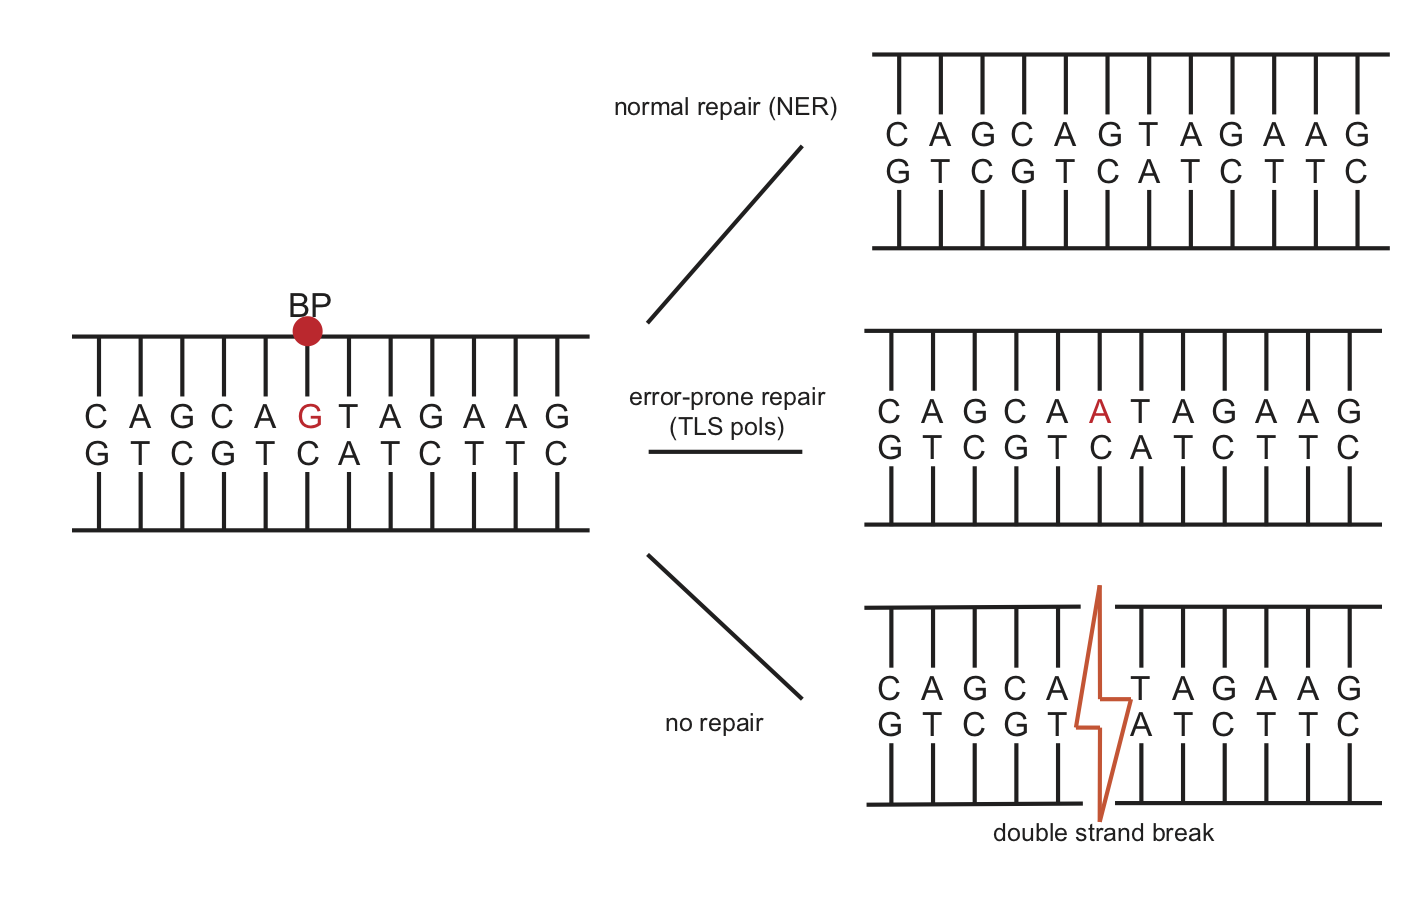
\includegraphics[width=1\textwidth]{figures/interaction_concept.png}}
  \caption{The precise type of mutation observed depends on the repair available. BP - Benzo-[a]-pyrene adduct.}
  \label{interaction_concept}
\end{figure}

\section{Quantifying interaction effects in a controlled experimental model}

The controlled nature of the mutagenesis screen allowed us to take a step further into dissection 
of contributions of DNA repair and DNA damage to the mutational spectra of \textit{C. elegans} samples.

Having the full information on the relative amount of exposure to each signature for each sample, it was possible to go beyond the recognition of the repetitive patterns and quantify the actual amount of change introduced by each interaction. Most of current mutagenesis models only account for non-negative effects: additional factors can only add mutations, but the data from certain experiments indicated that mutagenesis can in fact be reduced ***ref a figure from Chapter 2 here***. Hence the model should be able to reflect both amplification or reduction of existing signatures as well as transformation of genotoxin induced signatures.

In order to fulfill this task while maintaining interpretability of all model components, we developed a hierarchical Bayesian model which adapts all of the possible changes and noise sources in the data. 

\subsection{Bayesian modelling}

***TODO: why we used a hierarchical bayesian model***

For each of the mutation types $i$ and
samples $j$ we counted the respective number of mutations per sample $Y_{j,i}$.

As a first step, we use the mutation accumulation data to define a prior on signatures of DNA repair deficiencies, so that we could leverage the information from all mutant samples towards the refinement of signatures of genetic backgrounds. The posterior distribution will then be calculated using the rest of the samples. In the first stage, for each of the mutation accumulation samples, the mutation counts $Y \in \mathbb{R}_{+}^{119}$ were modeled by a negative binomial distribution,
\[Y \sim NB( \mu, \phi=100), \]
with expectation
\[ \mu = g \cdot G^{*} \cdot S_{G}^{*}.\]

Here $g$ denotes the adjusted generations in the absence of a mutagenic exposure as in Chapter 2. $G^{*}$ is a binary indicator matrix of genotypes, and $S_{G^{*}} \in Mat_{119\times51}(\mathbb{R}_{+})$ is a matrix of signatures of mutation accumulation effects per genotype (star denotes the subset of data where mutation accumulation data is available).

We used a log-normal prior distribution for these signatures, $S_{G^{*}} \sim logN(0, \sigma^{2}_{G})$ iid with a scalar variance $\sigma^{2}_{G}$. In total, we used 451 samples from mutation accumulation experiments with generation number higher than 1, and obtained signatures for 51 genotypes (\textit{agt-1}, \textit{exo-1}, \textit{rad-51} knockouts did not have mutation accumulation experiments).

In the next stage, the mutation counts for a given sample
$Y_{N,1:119}$ were modeled by a negative binomial distribution,

\[Y \sim \mathbb{NB} (\mu, \phi = 100), \]

with expectation
\[\mu = \mu_{G} \cdot (g + \alpha_{I}) + d \cdot \mu_{M} \cdot \beta_{I},\]

Here $\mu_{G} = G \times S_{G}^{T} \in \mathbb{R}_{2721\times119}^{+}$ describes 
the mutations expected due to the genetic background, with $G$ denoting an 
indicator matrix of genotypes per sample and $S_{G}$ being a matrix of 
mutational signatures of the genetic knockouts with a prior $S_{G} \sim \Gamma(shape_{G}, rate_{G})$ 
fitted to the posterior draws for $S_{G^{*}}$. 
Similarly, $\mu_{M} = M \cdot S_{M} \in \mathbb{R}^{+}_{2721 \times 119}$
is the expectation for the mutations created by mutagen M at median dose, 
with $M \in {0,1}^{2721 \times 12}$ being the indicator for the 12 mutagens 
used in this screen, and $S_{M} \in \mathbb{R}_{+}^{12\times119}$ being their 
signatures in wildtype, with per-column prior $S_{M}^{(j)} \sim logN\left(0, \sigma_{Mj}^2\right)$, where the variances $\sigma_{M}^2 = \left(\sigma_{M1}^2, ..., \sigma_{M12}^2\right)$ have prior distributions $\sigma_{Mj}^2 \sim \Gamma(1,1)$ iid. 
The terms $\alpha_{I} \in \mathbb{R}_{+}^{2721}$ and $\beta_{I} \in \mathbb{ℝ}_{+}^{196 \times 119}$ model how these terms interact. The scalar 
term for the genotype is linear with respect to the mutagen dose,

\[\alpha_{I} = d \cdot (I \cdot b_{I}) + (J \cdot a_{J}),\]

with $I \in {0,1}^{22721 \times 196}$ and $J \in {0,1}^{2721 × 208}$ being binary 
indicator matrices for all interactions and all mutagenesis experiments 
(i.e. interactions and wild-type mutagenesis experiments), respectively. 
Rates $b_{I} \in \mathbb{R}_{+}^{196}$  and offsets $a_{I} \in \mathbb{R}_{+}^{208}$ 
were modelled as log-normal distributed random variables,
$a_{I} \sim logN(0,0.5)$ and $b_{I} \sim logN(0,0.5)$. 
The rationale behind this parameterisation is that the \textit{C. elegans} 
strain used for the experiment may have slightly diverged, 
thereby adding $a_{I} \cdot S_{G}$ mutations with the same spectrum 
as in the absence of a mutagen. In addition to that, mutagen 
exposure can amplify the mutation types specific to the genotype, 
as in case of alkylating agent treatment of \textit{rev-3} deficient samples, 
and hence the mutagen exposure of dose d may add $d \cdot b_{I}$ mutations 
of the mutagen-free spectrum.

The main assumption about interaction effects is that the wild-type spectrum 
of the mutagen $S_M$ may change by the factors $\beta_{I} \in \mathbb{ℝ}_{+}^{119 \times 196}$ measuring the fold-change of each mutation type which is expressed as 

\[\beta_{I} = I \times S_{I},\] 

where $S_{I} \in \mathbb{R}_{+}^{196 \times 119}$ is the fold-change 
with 119 terms per interaction, with a prior distribution 
$log(S_I^{(j)}) \sim Laplace(0, \sigma_{Ij}^{2})$, all $\sigma_{Ij}^{2} \sim \Gamma(1,1)$ iid.

\subsection{Parameter estimation using Hamiltonian Monte-Carlo}

***TODO: about the HMC and convergence***

The overdispersion parameter $phi=100$ was selected based on the estimates of overdispersion in the dataset when fitting a negative binomial distribution with a shared overdispersion parameter to all the experiments in the dataset. It allows to account for additional variation within the replicates as well as for overflow of zeros which could present a problem in a Poisson framework.

The model was specified using R-package "greta" (Golding 2018), and the posteriors of $S_{G}$, $S_{M}$, $S_{I}$, $a_{J}$, $b_{I}$ and hyperparameters $\sigma^{2}_{M}$, $\sigma_{I}^{2}$ were estimated using Hamiltonian Monte Carlo sampling. We used 2000 steps for warmup and 5000 steps over 4 chains to ensure the best possible convergence. The point estimates for the parameters were taken as means of the samples across all chains. The relevant R codes are published on Github under \url{github.com/gerstung-lab/signature-interactions}.

EMS exposure was the only genotoxin for which we observed very different mutation counts across different experiments in wildtype. Respective samples were coming from 5 batches, which are stated in the ‘Comments’ section of the samples description table in Supplementary Table 1. In order to account for this effect, we introduced additional factor ={i}, i=1,...,4 which accounted for the log-difference in real dose applied to the samples in batches 2 to 5 compared to batch 1 which was considered as reference. The prior distribution for these adjustment was taken as iN(0,0.5)iid.  The dose for these samples was then calculated as d' = d*ebatch*, where batch{0,1}27214 is a binary matrix reflecting if a sample belongs to any of the batches 2-5. These adjustments were estimated along with the rest of the coefficients.

Combined genotype-mutagen interactions were tested for effect in two settings: altering the total number of base substitutions, and changing the distribution of mutations. The fold-change in the number of single base substitutions was calculated as predicted with interactions versus the one predicted without interactions using 2000 out of 10000 samples draws across 4 chains for all 196 interactions. The change in profile was quantified by calculating the cosine distance between the expected profiles with and without interactions, and those with distance higher than 0.2 were considered different. As all of the interactions which showed a change in signature appearance also came up in burden analysis, we only applied hypothesis testing (chi-square test for log(E(FCs))for s = 1, … 196) and Benjamini-Hochberg FDR control procedure for the set of substitution burden fold-changes.

%%%%%%%%%%

\section{Alteration of mutagen profiles in \textit{C. elegans} experiments}

\subsection{Alkylating agents and corresponding repair enzymes}

Among all of the interaction experiments, the higher number of mutations was observed for the knockout of TLS polymerase \textit{polk-1} under exposure to alkylating agents MMS and DMS. Absence of POLK-1 led to a 40x increased mutation rate per unit of genotoxin (1 mM for MMS, and 0.1 $\mu$M for DMS) as well as a visible change in the spectrum of mutations (Figure \ref{polk1mms}). T$>$A transversions increased $\sim 30$x, expecially in TpTpC and TpTpT contexts, and other mutation types including SNVs and MNVs were 10 times elevated. 

\begin{figure}[h]
  \centering
\centerline{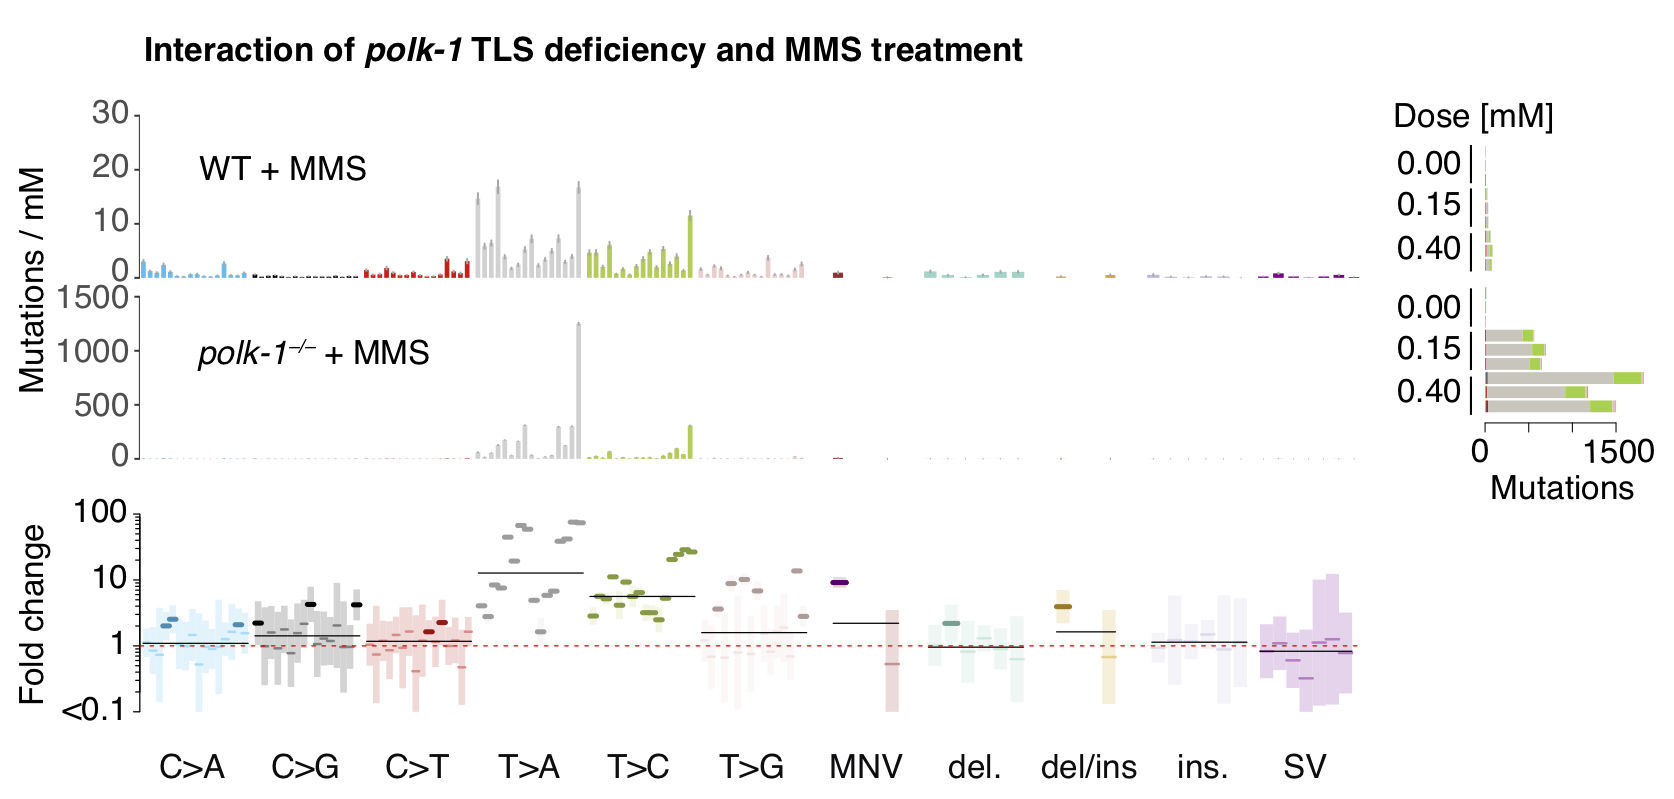
\includegraphics[width=1\textwidth]{figures/polk-1-MMS-interaction.png}}
  \caption{Mutations introduced per unit of MMS in wild-type (top panel) and in \textit{polk-1} deficient mutants (central panel), along with the fold-change per mutation type (bottom) and total numbers of mutation in response to different doses of mutagen (right panel).}
  \label{polk1mms}
\end{figure}


A similar change of the mutation spectrum was observed for DNA ethylation by EMS, however at a reduced rate of about 10x. This change in mutation spectrum reveal diverging repair of alkylated guanines and adenines: N3-methyladenosine, unlike O6-methylguanine, stalls replicative polymerases, which is overcome by TLS polymerase POLK-1, usually at the expense of fidelity, often incorporating false nucleotides9. Our data indicate that bypass by POLK-1 in wild type worms is relatively error free leading to the correct incorporation of a thymine on the opposing strand in most cases. Yet in the polk-1 mutant, bypass has to be achieved by other TLS polymerases, which results in increased T>N mutagenesis particularly favoring incorporation of an adenine leading to predominant of T$>$A mutations. 

Conversely, O6-methylguanine, another modification inflicted by the methylating agents MMS and DMS, leads to G:T mispairing resulting in C$>$T transitions and is repaired by distinct repair pathways. Knockout of the alkyl-transferase \textit{agt-1} increases C>T mutations by a factor of 4 under methylating MMS exposure, demonstrating that \textit{agt-1} removes most O6-methyl-guanine adducts error-free, thus acting as the functional C.elegans ortholog of the human methyl guanine methyl transferase MGMT. Interestingly, one observes a similar, but weaker interaction of \textit{agt-1} with the ethylation agent EMS, leading to an increase C>T transitions by a factor of 1.5, indicating that \textit{agt-1} is involved in, but less efficient at, removing ethyl groups. A knockout of the second alkyltransferase present in C. elegans, \textit{agt-2}, showed even smaller effect on O6-eG repair (increase by 20\% per average dose). Moreover, we also observe a uniformly increased MMS and DMS mutagenesis under knockouts of base excision repair (apn-1) and nucleotide excision repair (\textit{xpa-1}, \textit{xpf-1}; 1.2x and 2x, respectively), as well as a 1.2x increase of C$>$T mutations in mismatch repair knockout of \textit{mlh-1}, indicating that O6-meG:C pairs may be recognised and repaired by the components of these systems.

\subsection{Translesion synthesis and various mutagens}

Knockout of two other translesion polymerases, POLH-1 and REV-3, without exogeneous genotoxicity leads to a mutation pattern characterised by deletions in the range of 50-400 bp, thought to arise via the formation of DNA double strand breaks and \textit{polq-1} mediated repair. To protect the genome from such deleterious mutations, it is believed that TLS bypass such lesions at the cost of a higher base substitution rate. In line with this notion, we observed a 3-fold reduction in substitutions and 10-fold increase in indels in \textit{rev-3} knockouts under exposure with UV, and a 2-fold decrease in substitutions in \textit{polh-1} mutants under EMS exposure, indicating that DNA repair in some cases adds to overall mutagenicity.

\subsection{Nucleotide excision repair deficiency exaggerates the effects of mutagens}

In contrast to the the above examples where repair deficiency leads to both increase in mutagenesis but also to alteration of mutational spectra, the knockouts of the NER genes \textit{xpf-1} and \textit{xpc-1} increased the rate of UV-B induced mutagenesis by factors of 10 and 35, respectively. The fold-change appears to be relatively uniform across the entire mutation spectrum, indicating that NER is involved in repairing the large majority of UV-B damage of different types, including both single- and multinucleotide lesions (Fig. 3g). Interestingly, \textit{xpf-1} knockout also uniformly increased the mutation burden due to alkylation by a factor of 2 indicating that alkylation damage is eventually repaired by NER. Similarly \textit{xpf-1} knockouts also showed an two-fold increase in mutations after aristolochic acid, demonstrating that NER repairs both small and bulky adducts.


\subsection{Widespread interaction effects across the screen and mutation summary}

These examples of genotoxin-repair interactions are not uncommon: In total, 72/196 (37\%, at FDR of 10\%) of combinations displayed an interaction between DNA repair status and genotoxin treatment. Conversely, more than half of combinations produced mutation spectra which could be fully described as the superposition of the wild-type genotoxin signature and that of the DNA repair deficiency background, indicating that the two processes acted independently. Usually genotoxin-repair interactions increase the numbers of mutations obtained for a given dose of mutagen, leaving the mutational spectrum mostly unchanged, others have a profound impact on mutational spectra (Figure 4B, for a comprehensive list of effects see Supplementary Figure 5 and Supplementary Table 3). The emergence of distinct mutational spectra depending on DNA repair status reflects how multiple repair enzymes and pathways contribute to mending damaged DNA as in the case of DNA alkylation. If DNA repair is predominantly achieved by one pathway such as by NER for UVB damage and bulky DNA adducts, the number of mutations is increased, but the signature tends to remain unchanged.

To illustrate the overall magnitude of these interaction effects, we estimate that of the 141,004 mutations we observed upon treatment with genotoxins in DNA repair deficient strains 23\% of mutations were attributed to the endogenous mutagenicity of DNA repair deficiency genotypes independent of genotoxic exposure, and 62\% of mutations would be attributed to genotoxic exposures independent of the genetic background. Of these, 2\% were not observed due to negative interactions of genotoxins and DNA repair deficiency, such as UVB exposure of TLS knockout strains, and 17\% of mutations were added because of the positive interactions, which increased mutagenicity.

In summary, the above examples and analysis demonstrate that the combination of DNA damage and DNA repair deficiency can yield mutational patterns which can not be explained by the mere superposition of patterns resulting from exposure of wild-type DNA repair proficient strains and mutagenesis induced in repair defective strains in the absence of external mutagenesis. The alteration of mutational pattern by DNA repair status appears most remarkable when multiple repair enzymes and pathways contribute to mend damaged DNA as in the case of DNA alkylation. If repair is predominantly affected by one pathway such as NER for UV damage and bulky DNA adducts, the number of mutations is increased but the spectrum tends to remain unchanged.

\subsubsection*{Evidence of interactions from other sources}

Data from other model experiments???

Metabolic activation of mutagens in mammals???


%%%%%%%%%%%%%%%%%%%%%%%%%%%%%%%%%%%%%%%%%%

\section{Discussion}

In this chapter, I presented a way of quantifying the degree of interaction between
genetic and mutagenic factors in controlled experiments on \textit{C. elegans}, and performed
a comparison of effects across 196 combinations of repair components and damaging agents
which showed the diversity and abundance of significant interaction effects which may
be both positive and negative. I also demonstrated how these interactions may increase
or decrease the total burden, and they may alter the signature of the mutagenic agent
as well as intensify the signature of genetic factors.

This analysis shows that the signatures of many mutagenic processes are not necessarily
consistent: depending on the DNA repair availability, their contributions will be different
and not aligned with the exposure dose, and their mutational spectra can change partially or
completely. It opens the way for considering DNA repair status as a factor in signature
decomposition as it may alter the appearance of latent components or introduce additional ones.

Studying the effects of DNA repair deficiencies on the mutagenic exposures also provides
insights into the mechanisms of repair and specificity of the damage. The screen above only
considers mutations, i.e. results of repair-damage interplay; combined with the analysis
of unrepaired damage, which may be detected with direct damage detection methods including
Nanopore sequencing and other techniques, it could provide a comprehensive and quantitative
picture of mechanisms of damage and repair of the genomic DNA.

Another limitations which needs to be taken into account is the simplicity of mutagen intake
in \textit{C. elegans} which does not necessarily correspond to the processing applied upon 
mutagenic agents in human body, as was mentioned in the Chapter 1. Metabolic activation, 
differences in sensitivity or repair across tissues, or other ways of substance 
processing may completely alter mutagenic activity of certain agents or of the repair activity,
hence a further investigation of these effects in human cells and organs deems necessary.

In the next chapter, I will explore the range of repair-damage interaction in human
cancers by modifying the signature extraction model and incorporating additional information
about DNA repair status of the samples.

\end{document}





